\section{Task 2, Inverted Pendulum}
% Task A
\subsection{Task A}
\textbf{\textit{Task: By observing the transfer function $P_{pend}$(s), determine whether the system is stable, unstable,
or marginally stable. Explain your answer!}}

\begin{equation*}
    TF = \frac{0.01s}{s^3 + 10.1s^2-s-10}
\end{equation*}

The system is unstable because the system has two negative numbers in the denominator. The only way that the denominator can be factored is if it has at least one factor on the form of (s - a). This means that at least one pole is on the positive side of the X axis.

% Task B
\subsection{Task B}
\textbf{\textit{Task: Determine the location of the poles using Routh-Hurwitz criterion.}}

The Routh-Hurwitx calculations show that the system has one positive and two negative poles.

\begin{figure}[h]
    \centering
    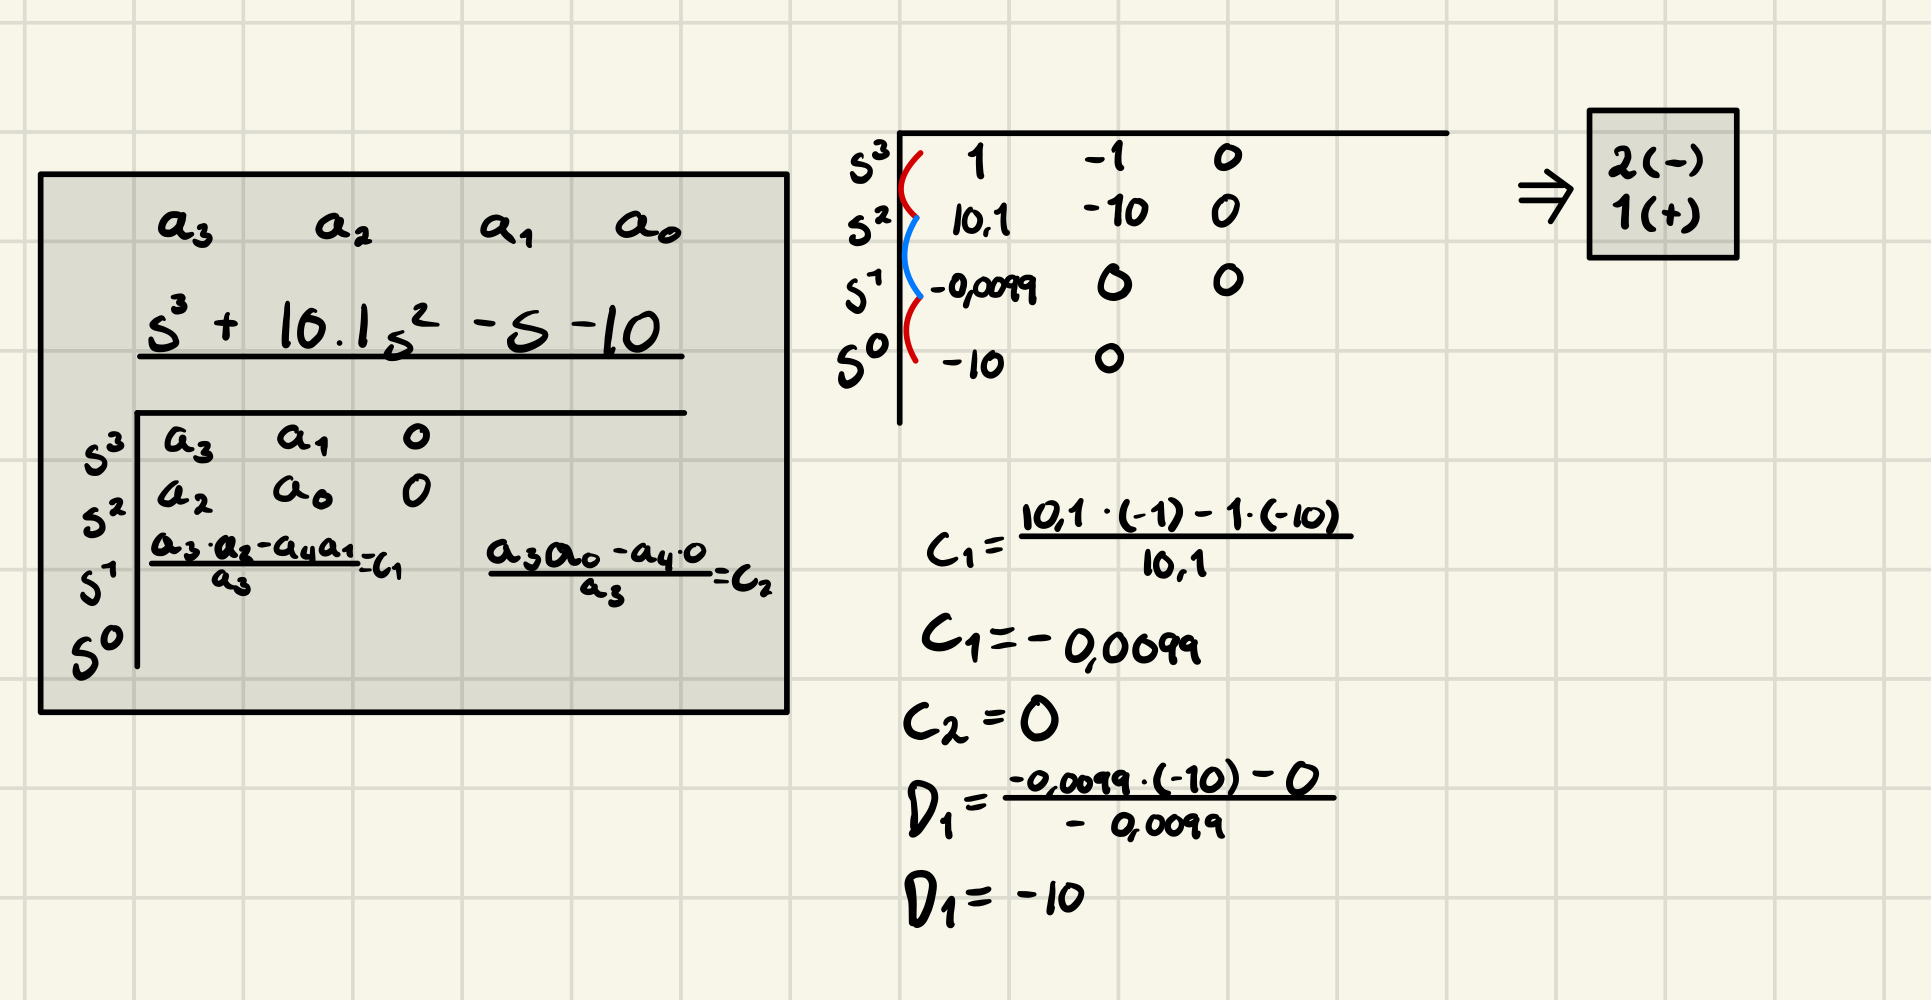
\includegraphics[width = 0.8\textwidth]{Images/2B_Calc.jpeg}
    \caption{Calculations of Routh-Hurwitz criterion.}
    \label{fig:2B_Calc}
\end{figure}


% Task C
\subsection{Task C}
\textbf{\textit{Task: Use Matlab to find the location of the poles.}}
\newline
\textit{Code: \ref{apx:2C_matlab}}


The system is unstable due to one of the poles being positive.
MATLAB gave the following answer when calculating the poles.
\begin{align*}
        P1 =& -10.1010 \\
        P2 =& 0.9955 \\
        P3 =& -0.9945
\end{align*}


% Task D
\subsection{Task D}
\textbf{\textit{Task:  Find the closed-loop transfer function of the unity feedback system.}}
\newline
\textit{Code: \ref{apx:2D_matlab}}

\begin{equation*}
    P_{CL} = \frac{0.01 s}{s^3 + 10.01 s^2 - 0.99 s - 10}
\end{equation*}


% Task E
\subsection{Task E}
\textbf{\textit{Task: Plot the root locus for the transfer function $P_{pend}$(s).}}

\textit{Code: \ref{apx:2E_matlab}}

\begin{figure}[h!]
    \centering
    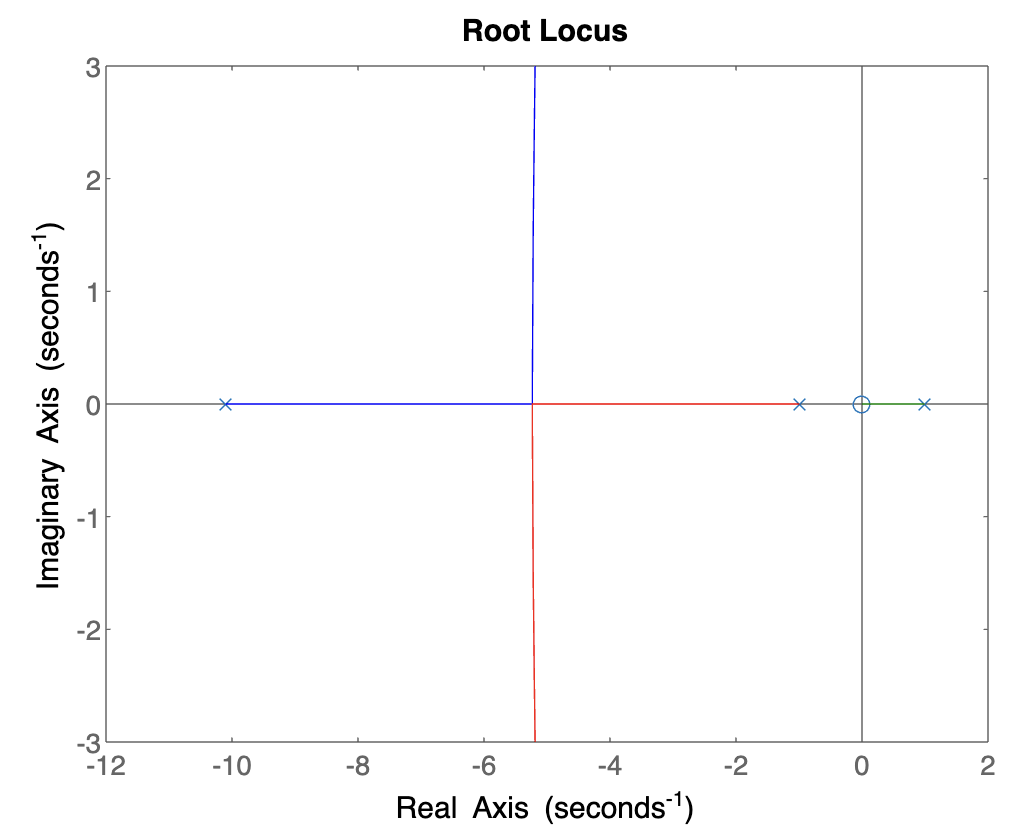
\includegraphics[width = 0.8\textwidth]{Images/2E_Rlocus.png}
    \caption{Rlocus for the transfer function.}
    \label{fig:2E_Rlocus}
\end{figure}

% Task F
\subsection{Task F}
\textbf{\textit{Task: Design a PI controller that can stabilize the closed-loop system.}}
\newline
\textit{Code: \ref{apx:2F_matlab}}

\begin{equation}
    G = \frac{100s + 200}{s}
    \label{fig:PI2}
\end{equation}

\begin{equation}
    TF = \frac{G(s)}{1+G(s)} = \frac{\frac{n}{m}}{1+\frac{n}{m}} = \frac{n(s)}{m(s)+n(s)}
\end{equation}

Because one pole is in the positive side of the X axis, the values that were chosen for Kp and Ki were very large.
The PI that was initially chosen was $\frac {100s + 200}{s}$. 
\newline
The gain was found by looking at the root locus of the system at 10 \%. After taking the gain of 30.6 into consideration for the system the systems step response was stable. Figure \ref{fig:PI2} show the new step response after the PI controller is added. Kp = 100, Ki = 200, k = 30.6.

\begin{equation}
    PI = 30.6 \cdot \frac{100s + 200}{s}
    \label{fig:PI2}
\end{equation}

\begin{figure}[h!]
    \centering
    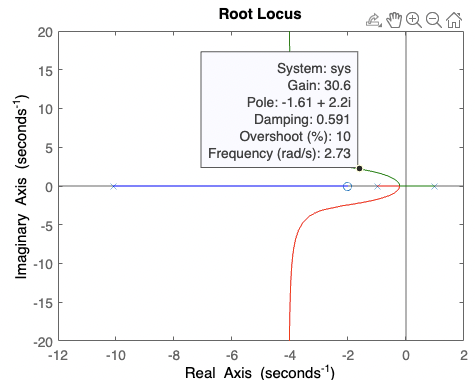
\includegraphics[width = 0.8\textwidth]{Images/2F_Rlocus.png}
    \caption{Rlocus of system without PI controller.}
    \label{fig:2F_Rlocus}
\end{figure}

% Task G
\subsection{Task G}
\textbf{\textit{Task: Plot the step response (likely you still have steady state error).}}
\newline
\textit{Code: \ref{apx:2G_matlab}}

\begin{figure}[h!]
    \centering
    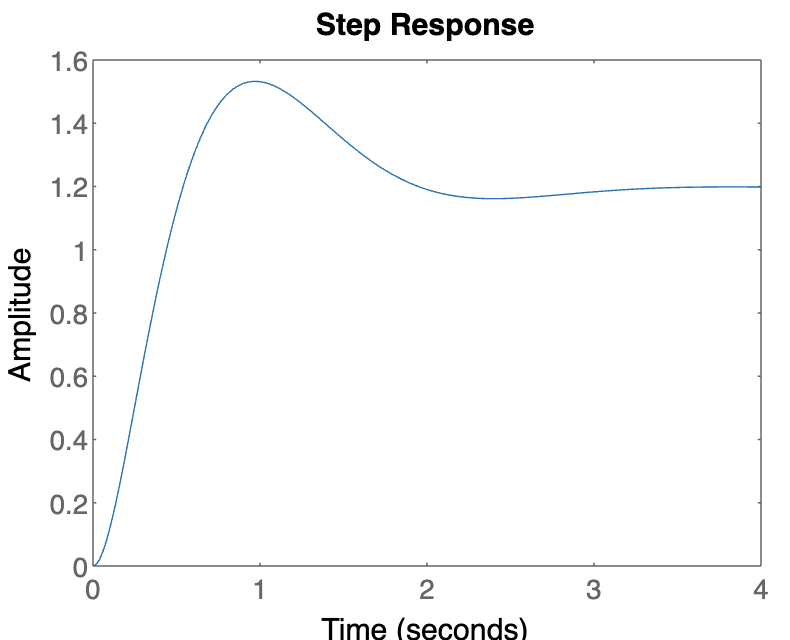
\includegraphics[width = 0.8\textwidth]{Images/2G_Step.png}
    \caption{Step response of system with PI controller.}
    \label{fig:2G_Step}
\end{figure}

% Task H
\subsection{Task H}
\textbf{\textit{Task: Calculate the DC gain ($K_{DC}$) of the closed-loop system using the following formula:}}
\begin{equation}
    K_{DC} = \lim_{s \to 0} G(s)
\end{equation}
\textbf{\textit{where G(s) is the transfer function of the closed-loop system. The pre-compensation is given
by $\overline{N} = \frac {1}{K_{DC}}$.}}


\begin{align*}
     K_{DC} =&  \lim_{s \to 0} \frac{30.6s^4 + 370.3s^3 + 587.5s^2 - 367.2s - 612}{s^6 + 20.2s^5 + 130.6s^4 + 330.1s^3 + 386.5s^2 - 347.2s - 512} \\
     \newline
     K_{DC} =&  \frac{612}{512} \\
     \newline
     K_{DC} =& 1.19531 \\
     \newline
\end{align*}

\begin{align*}
    \overline{N} =& \frac{1}{K_{DC}} \\
     \newline
     \overline{N} =& \frac{1}{1.19531} \\
     \newline
     \overline{N} =& 0.8366
\end{align*}

% Task I
\subsection{Task I}
\textbf{\textit{Task: Multiply the pre-compensation with the input and plot the result.}}
\newline
\textit{Code: \ref{apx:2I_matlab}}

\begin{figure}[h!]
    \centering
    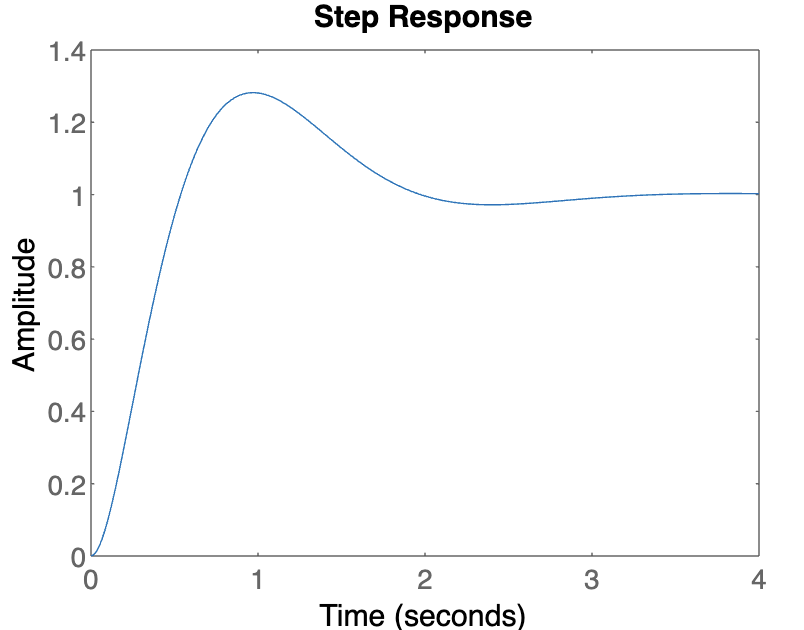
\includegraphics[width = 0.8\textwidth]{Images/2I_Step.png}
    \caption{Step response of system with PI and pre-compensator.}
    \label{fig:2I_Step}
\end{figure}